\documentclass{whiteboard}
\begin{document}
\begin{frame}[plain,t]
\bbcover{Combinadores}{Introdução}{Prof. Edson Alves}{Campus UnB Gama: Faculdade de Ciências e Tecnologias em Engenharia}

\end{frame}
\begin{frame}[plain,t]
\begin{tikzpicture}
\node[draw,opacity=0] at (0, 0) {x};
\node[draw,opacity=0] at (14, 8) {x};

	\node[anchor=west] (title) at (0.0, 7.0) { \Large \bbbold{Moses Schönfinkel} };

	\node[] (moses) at (3.0, 4.0) { 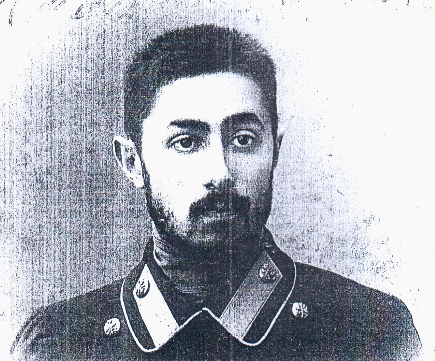
\includegraphics[scale=0.3]{figs/moses2.png} };

	\node[anchor=west] (flag) at (1.2, 1.5) { 
\includegraphics[scale=0.015]{figs/ucrania.png} };

	\node[] (dates) at (3.5, 1.5) { * \bbtext{1889} \hspace*{0.05in} \bbtext{\textdagger\ 1942} };

\end{tikzpicture}
\end{frame}
\begin{frame}[plain,t]
\begin{tikzpicture}
\node[draw,opacity=0] at (0, 0) {x};
\node[draw,opacity=0] at (14, 8) {x};

	\node[anchor=west] (title) at (0.0, 7.0) { \Large \bbbold{Moses Schönfinkel} };

	\node[] (moses) at (3.0, 4.0) { 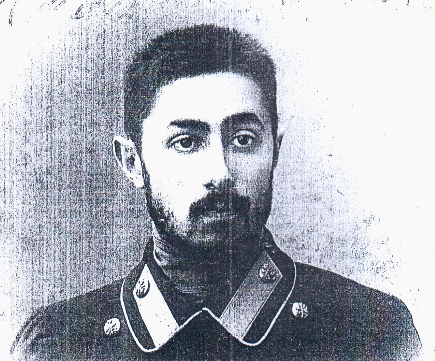
\includegraphics[scale=0.3]{figs/moses2.png} };

	\node[anchor=west] (flag) at (1.2, 1.5) { 
\includegraphics[scale=0.015]{figs/ucrania.png} };

	\node[] (dates) at (3.5, 1.5) { * \bbtext{1889} \hspace*{0.05in} \bbtext{\textdagger\ 1942} };


	\node[anchor=west] (article) at (6.0, 6.0) { \large {\bbnote{On the building blocks of mathematical logic}} };

\end{tikzpicture}
\end{frame}
\begin{frame}[plain,t]
\begin{tikzpicture}
\node[draw,opacity=0] at (0, 0) {x};
\node[draw,opacity=0] at (14, 8) {x};

	\node[anchor=west] (title) at (0.0, 7.0) { \Large \bbbold{Moses Schönfinkel} };

	\node[] (moses) at (3.0, 4.0) { 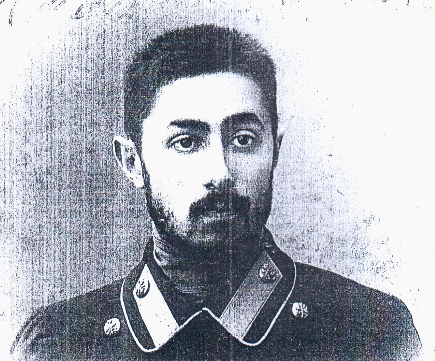
\includegraphics[scale=0.3]{figs/moses2.png} };

	\node[anchor=west] (flag) at (1.2, 1.5) { 
\includegraphics[scale=0.015]{figs/ucrania.png} };

	\node[] (dates) at (3.5, 1.5) { * \bbtext{1889} \hspace*{0.05in} \bbtext{\textdagger\ 1942} };


	\node[anchor=west] (article) at (6.0, 6.0) { \large {\bbnote{On the building blocks of mathematical logic}} };


	\node[anchor=west] (a) at (6.5, 5.0) { $\star$ \bbtext{As ideias foram apresentadas em 1920} };

\end{tikzpicture}
\end{frame}
\begin{frame}[plain,t]
\begin{tikzpicture}
\node[draw,opacity=0] at (0, 0) {x};
\node[draw,opacity=0] at (14, 8) {x};

	\node[anchor=west] (title) at (0.0, 7.0) { \Large \bbbold{Moses Schönfinkel} };

	\node[] (moses) at (3.0, 4.0) { 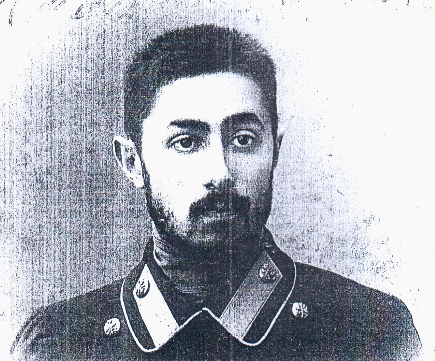
\includegraphics[scale=0.3]{figs/moses2.png} };

	\node[anchor=west] (flag) at (1.2, 1.5) { 
\includegraphics[scale=0.015]{figs/ucrania.png} };

	\node[] (dates) at (3.5, 1.5) { * \bbtext{1889} \hspace*{0.05in} \bbtext{\textdagger\ 1942} };


	\node[anchor=west] (article) at (6.0, 6.0) { \large {\bbnote{On the building blocks of mathematical logic}} };


	\node[anchor=west] (a) at (6.5, 5.0) { $\star$ \bbtext{As ideias foram apresentadas em 1920} };


	\node[anchor=west] (b) at (6.5, 4.0) { $\star$ \bbtext{O artigo foi publicado em 1924} };

\end{tikzpicture}
\end{frame}
\begin{frame}[plain,t]
\begin{tikzpicture}
\node[draw,opacity=0] at (0, 0) {x};
\node[draw,opacity=0] at (14, 8) {x};

	\node[anchor=west] (title) at (0.0, 7.0) { \Large \bbbold{Moses Schönfinkel} };

	\node[] (moses) at (3.0, 4.0) { 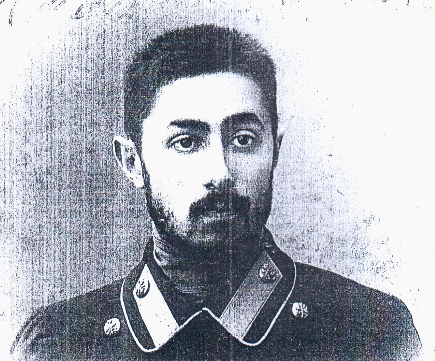
\includegraphics[scale=0.3]{figs/moses2.png} };

	\node[anchor=west] (flag) at (1.2, 1.5) { 
\includegraphics[scale=0.015]{figs/ucrania.png} };

	\node[] (dates) at (3.5, 1.5) { * \bbtext{1889} \hspace*{0.05in} \bbtext{\textdagger\ 1942} };


	\node[anchor=west] (article) at (6.0, 6.0) { \large {\bbnote{On the building blocks of mathematical logic}} };


	\node[anchor=west] (a) at (6.5, 5.0) { $\star$ \bbtext{As ideias foram apresentadas em 1920} };


	\node[anchor=west] (b) at (6.5, 4.0) { $\star$ \bbtext{O artigo foi publicado em 1924} };


	\node[anchor=west] (c) at (6.5, 3.0) { $\star$ \bbtext{Introduziu os combinadores} };

\end{tikzpicture}
\end{frame}
\begin{frame}[plain,t]
\begin{tikzpicture}
\node[draw,opacity=0] at (0, 0) {x};
\node[draw,opacity=0] at (14, 8) {x};

	\node[anchor=west] (title) at (0.0, 7.0) { \Large \bbbold{Moses Schönfinkel} };

	\node[] (moses) at (3.0, 4.0) { 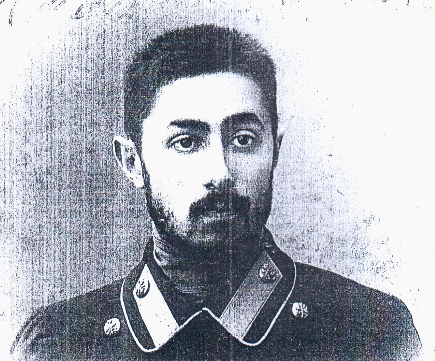
\includegraphics[scale=0.3]{figs/moses2.png} };

	\node[anchor=west] (flag) at (1.2, 1.5) { 
\includegraphics[scale=0.015]{figs/ucrania.png} };

	\node[] (dates) at (3.5, 1.5) { * \bbtext{1889} \hspace*{0.05in} \bbtext{\textdagger\ 1942} };


	\node[anchor=west] (article) at (6.0, 6.0) { \large {\bbnote{On the building blocks of mathematical logic}} };


	\node[anchor=west] (a) at (6.5, 5.0) { $\star$ \bbtext{As ideias foram apresentadas em 1920} };


	\node[anchor=west] (b) at (6.5, 4.0) { $\star$ \bbtext{O artigo foi publicado em 1924} };


	\node[anchor=west] (c) at (6.5, 3.0) { $\star$ \bbtext{Introduziu os combinadores} };


	\node[anchor=west] (d) at (6.5, 2.0) { $\star$ \bbtext{Resgatou a ideia de Frege (1893) de tratar} };

	\node[anchor=west] (d1) at (6.0, 1.4) { \bbtext{todas as funções como unárias (\bbenglish{currying})} };

\end{tikzpicture}
\end{frame}
\begin{frame}[plain,t]
\begin{tikzpicture}
\node[draw,opacity=0] at (0, 0) {x};
\node[draw,opacity=0] at (14, 8) {x};

	\node[anchor=west] (title) at (0.0, 7.0) { \Large \bbbold{Conectivos da lógica proposicional booleana} };

\end{tikzpicture}
\end{frame}
\begin{frame}[plain,t]
\begin{tikzpicture}
\node[draw,opacity=0] at (0, 0) {x};
\node[draw,opacity=0] at (14, 8) {x};

	\node[anchor=west] (title) at (0.0, 7.0) { \Large \bbbold{Conectivos da lógica proposicional booleana} };


	\draw[very thick] (0.0, 6.0) to  (13.0, 6.0);

	\draw[thick] (0.0, 5.0) to  (13.0, 5.0);

	\node[anchor=west] (op) at (0.25, 5.5) { \bbemph{Operação$^1$} };

	\node[anchor=west] (read) at (3.0, 5.5) { \bbemph{Leitura} };

	\node[anchor=west] (desc) at (5.5, 5.5) { \bbemph{Definição} };

\end{tikzpicture}
\end{frame}
\begin{frame}[plain,t]
\begin{tikzpicture}
\node[draw,opacity=0] at (0, 0) {x};
\node[draw,opacity=0] at (14, 8) {x};

	\node[anchor=west] (title) at (0.0, 7.0) { \Large \bbbold{Conectivos da lógica proposicional booleana} };


	\draw[very thick] (0.0, 6.0) to  (13.0, 6.0);

	\draw[thick] (0.0, 5.0) to  (13.0, 5.0);

	\node[anchor=west] (op) at (0.25, 5.5) { \bbemph{Operação$^1$} };

	\node[anchor=west] (read) at (3.0, 5.5) { \bbemph{Leitura} };

	\node[anchor=west] (desc) at (5.5, 5.5) { \bbemph{Definição} };


	\node[] (not) at (1.2, 4.5) { $\bar{a}$ };

	\node[] (not_read) at (3.8, 4.5) { \footnotesize \bbtext{não $a$} };

	\node[anchor=west] (not_desc) at (5.5, 4.5) { \footnotesize \bbtext{Inverte o valor lógico de $a$} };

\end{tikzpicture}
\end{frame}
\begin{frame}[plain,t]
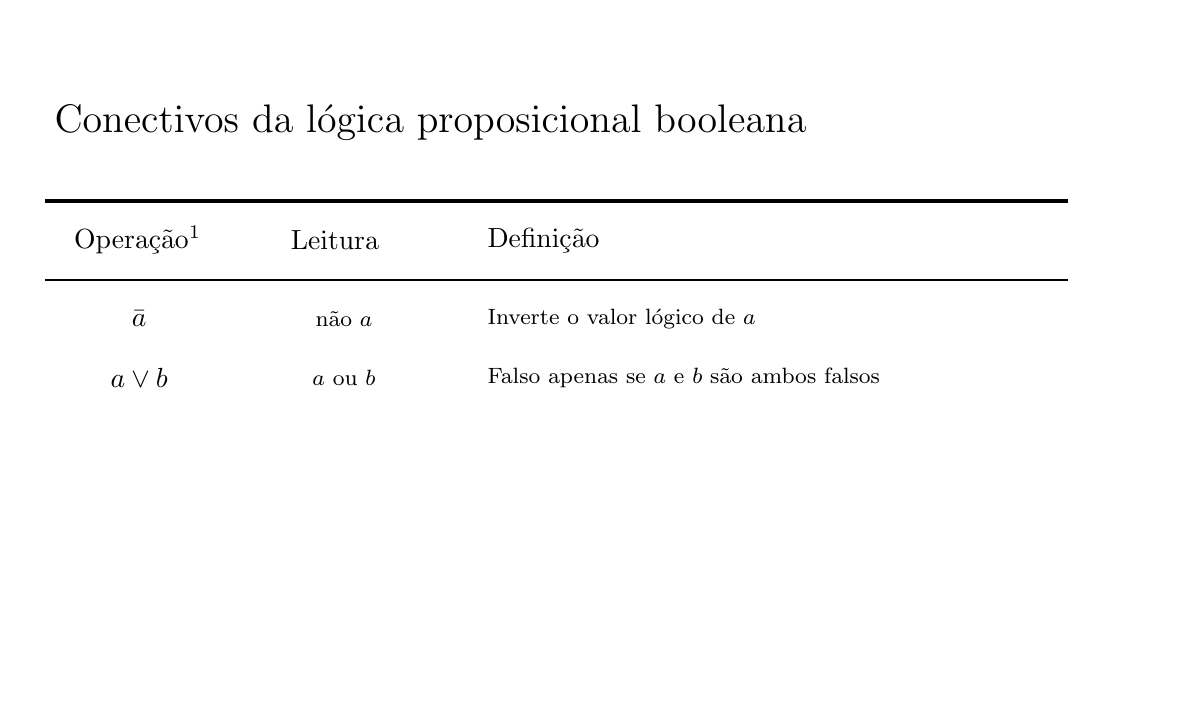
\begin{tikzpicture}
\node[draw,opacity=0] at (0, 0) {x};
\node[draw,opacity=0] at (14, 8) {x};

	\node[anchor=west] (title) at (0.0, 7.0) { \Large \bbbold{Conectivos da lógica proposicional booleana} };


	\draw[very thick] (0.0, 6.0) to  (13.0, 6.0);

	\draw[thick] (0.0, 5.0) to  (13.0, 5.0);

	\node[anchor=west] (op) at (0.25, 5.5) { \bbemph{Operação$^1$} };

	\node[anchor=west] (read) at (3.0, 5.5) { \bbemph{Leitura} };

	\node[anchor=west] (desc) at (5.5, 5.5) { \bbemph{Definição} };


	\node[] (not) at (1.2, 4.5) { $\bar{a}$ };

	\node[] (not_read) at (3.8, 4.5) { \footnotesize \bbtext{não $a$} };

	\node[anchor=west] (not_desc) at (5.5, 4.5) { \footnotesize \bbtext{Inverte o valor lógico de $a$} };


	\node[] (or) at (1.2, 3.75) { $a\vee b$ };

	\node[] (or_read) at (3.8, 3.75) { \footnotesize \bbtext{$a$ ou $b$} };

	\node[anchor=west] (or_desc) at (5.5, 3.75) { \footnotesize \bbtext{Falso apenas se $a$ e $b$ são ambos falsos} };

\end{tikzpicture}
\end{frame}
\begin{frame}[plain,t]
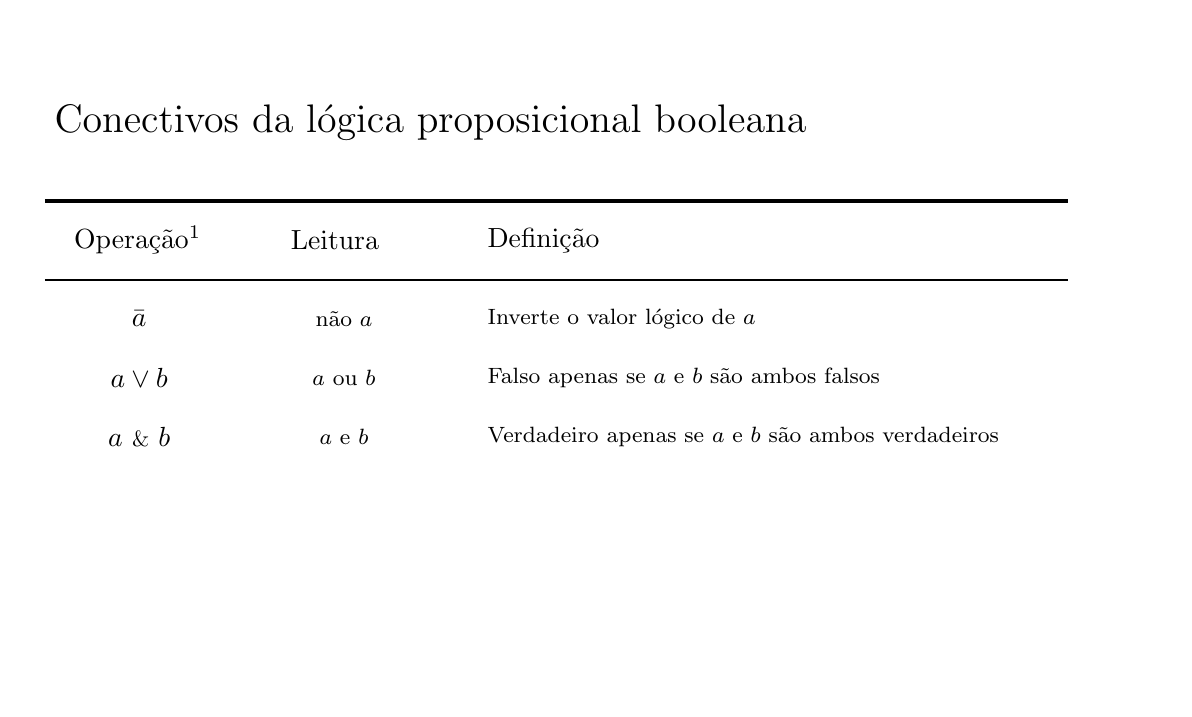
\begin{tikzpicture}
\node[draw,opacity=0] at (0, 0) {x};
\node[draw,opacity=0] at (14, 8) {x};

	\node[anchor=west] (title) at (0.0, 7.0) { \Large \bbbold{Conectivos da lógica proposicional booleana} };


	\draw[very thick] (0.0, 6.0) to  (13.0, 6.0);

	\draw[thick] (0.0, 5.0) to  (13.0, 5.0);

	\node[anchor=west] (op) at (0.25, 5.5) { \bbemph{Operação$^1$} };

	\node[anchor=west] (read) at (3.0, 5.5) { \bbemph{Leitura} };

	\node[anchor=west] (desc) at (5.5, 5.5) { \bbemph{Definição} };


	\node[] (not) at (1.2, 4.5) { $\bar{a}$ };

	\node[] (not_read) at (3.8, 4.5) { \footnotesize \bbtext{não $a$} };

	\node[anchor=west] (not_desc) at (5.5, 4.5) { \footnotesize \bbtext{Inverte o valor lógico de $a$} };


	\node[] (or) at (1.2, 3.75) { $a\vee b$ };

	\node[] (or_read) at (3.8, 3.75) { \footnotesize \bbtext{$a$ ou $b$} };

	\node[anchor=west] (or_desc) at (5.5, 3.75) { \footnotesize \bbtext{Falso apenas se $a$ e $b$ são ambos falsos} };


	\node[] (and) at (1.2, 3.0) { $a\ \scalebox{0.8}\&\  b$ };

	\node[] (and_read) at (3.8, 3.0) { \footnotesize \bbtext{$a$ e $b$} };

	\node[anchor=west] (and_desc) at (5.5, 3.0) { \footnotesize \bbtext{Verdadeiro apenas se $a$ e $b$ são ambos verdadeiros} };

\end{tikzpicture}
\end{frame}
\begin{frame}[plain,t]
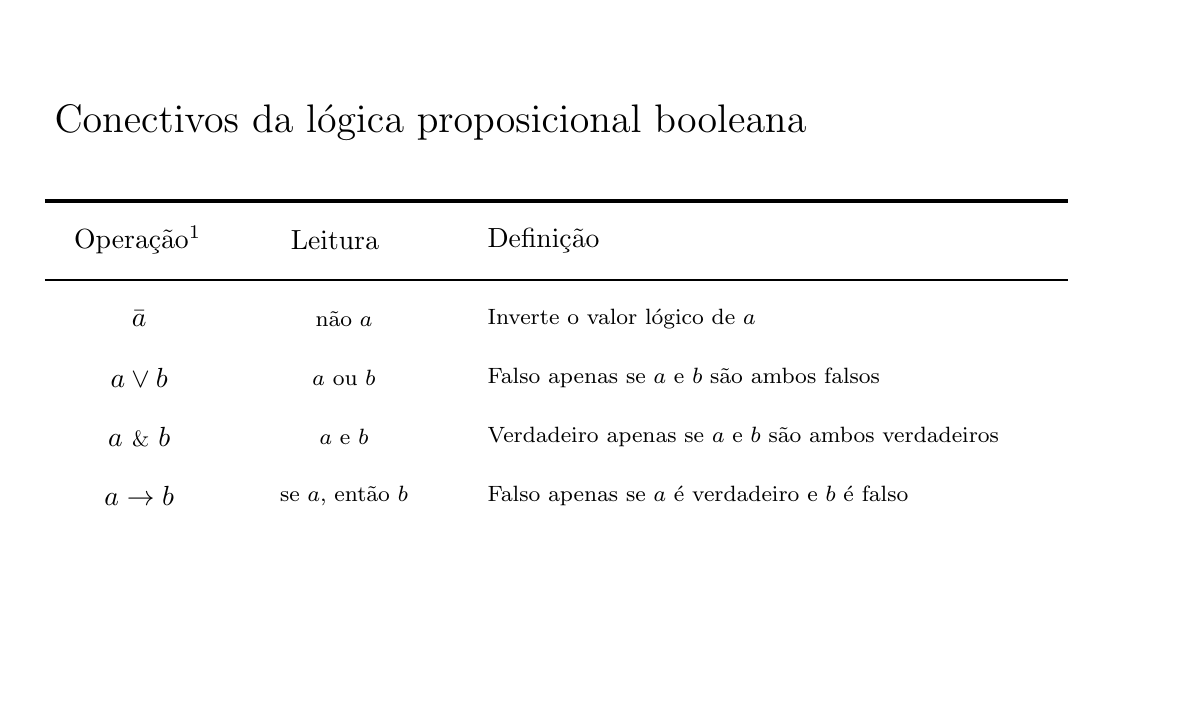
\begin{tikzpicture}
\node[draw,opacity=0] at (0, 0) {x};
\node[draw,opacity=0] at (14, 8) {x};

	\node[anchor=west] (title) at (0.0, 7.0) { \Large \bbbold{Conectivos da lógica proposicional booleana} };


	\draw[very thick] (0.0, 6.0) to  (13.0, 6.0);

	\draw[thick] (0.0, 5.0) to  (13.0, 5.0);

	\node[anchor=west] (op) at (0.25, 5.5) { \bbemph{Operação$^1$} };

	\node[anchor=west] (read) at (3.0, 5.5) { \bbemph{Leitura} };

	\node[anchor=west] (desc) at (5.5, 5.5) { \bbemph{Definição} };


	\node[] (not) at (1.2, 4.5) { $\bar{a}$ };

	\node[] (not_read) at (3.8, 4.5) { \footnotesize \bbtext{não $a$} };

	\node[anchor=west] (not_desc) at (5.5, 4.5) { \footnotesize \bbtext{Inverte o valor lógico de $a$} };


	\node[] (or) at (1.2, 3.75) { $a\vee b$ };

	\node[] (or_read) at (3.8, 3.75) { \footnotesize \bbtext{$a$ ou $b$} };

	\node[anchor=west] (or_desc) at (5.5, 3.75) { \footnotesize \bbtext{Falso apenas se $a$ e $b$ são ambos falsos} };


	\node[] (and) at (1.2, 3.0) { $a\ \scalebox{0.8}\&\  b$ };

	\node[] (and_read) at (3.8, 3.0) { \footnotesize \bbtext{$a$ e $b$} };

	\node[anchor=west] (and_desc) at (5.5, 3.0) { \footnotesize \bbtext{Verdadeiro apenas se $a$ e $b$ são ambos verdadeiros} };


	\node[] (conditional) at (1.2, 2.25) { $a \to  b$ };

	\node[] (conditional_read) at (3.8, 2.25) { \footnotesize \bbtext{se $a$, então $b$} };

	\node[anchor=west] (conditional_desc) at (5.5, 2.25) { \footnotesize \bbtext{Falso apenas se $a$ é verdadeiro e $b$ é falso} };

\end{tikzpicture}
\end{frame}
\begin{frame}[plain,t]
\begin{tikzpicture}
\node[draw,opacity=0] at (0, 0) {x};
\node[draw,opacity=0] at (14, 8) {x};

	\node[anchor=west] (title) at (0.0, 7.0) { \Large \bbbold{Conectivos da lógica proposicional booleana} };


	\draw[very thick] (0.0, 6.0) to  (13.0, 6.0);

	\draw[thick] (0.0, 5.0) to  (13.0, 5.0);

	\node[anchor=west] (op) at (0.25, 5.5) { \bbemph{Operação$^1$} };

	\node[anchor=west] (read) at (3.0, 5.5) { \bbemph{Leitura} };

	\node[anchor=west] (desc) at (5.5, 5.5) { \bbemph{Definição} };


	\node[] (not) at (1.2, 4.5) { $\bar{a}$ };

	\node[] (not_read) at (3.8, 4.5) { \footnotesize \bbtext{não $a$} };

	\node[anchor=west] (not_desc) at (5.5, 4.5) { \footnotesize \bbtext{Inverte o valor lógico de $a$} };


	\node[] (or) at (1.2, 3.75) { $a\vee b$ };

	\node[] (or_read) at (3.8, 3.75) { \footnotesize \bbtext{$a$ ou $b$} };

	\node[anchor=west] (or_desc) at (5.5, 3.75) { \footnotesize \bbtext{Falso apenas se $a$ e $b$ são ambos falsos} };


	\node[] (and) at (1.2, 3.0) { $a\ \scalebox{0.8}\&\  b$ };

	\node[] (and_read) at (3.8, 3.0) { \footnotesize \bbtext{$a$ e $b$} };

	\node[anchor=west] (and_desc) at (5.5, 3.0) { \footnotesize \bbtext{Verdadeiro apenas se $a$ e $b$ são ambos verdadeiros} };


	\node[] (conditional) at (1.2, 2.25) { $a \to  b$ };

	\node[] (conditional_read) at (3.8, 2.25) { \footnotesize \bbtext{se $a$, então $b$} };

	\node[anchor=west] (conditional_desc) at (5.5, 2.25) { \footnotesize \bbtext{Falso apenas se $a$ é verdadeiro e $b$ é falso} };


	\node[] (equivalence) at (1.2, 1.5) { $a\ \scalebox{1.2}[0.8]{\sim}\ b$ };

	\node[] (equivalence_read) at (3.8, 1.5) { \footnotesize \bbtext{$a$ é equivalente a $b$} };

	\node[anchor=west] (equivalence_desc) at (5.5, 1.5) { \footnotesize \bbtext{Verdadeiro se ambos tem mesmo valor lógico} };


	\draw[very thick] (0.0, 1.0) to  (13.0, 1.0);

\end{tikzpicture}
\end{frame}
\begin{frame}[plain,t]
\begin{tikzpicture}
\node[draw,opacity=0] at (0, 0) {x};
\node[draw,opacity=0] at (14, 8) {x};

	\node[anchor=west] (title) at (0.0, 7.0) { \Large \bbbold{Conectivos da lógica proposicional booleana} };


	\draw[very thick] (0.0, 6.0) to  (13.0, 6.0);

	\draw[thick] (0.0, 5.0) to  (13.0, 5.0);

	\node[anchor=west] (op) at (0.25, 5.5) { \bbemph{Operação$^1$} };

	\node[anchor=west] (read) at (3.0, 5.5) { \bbemph{Leitura} };

	\node[anchor=west] (desc) at (5.5, 5.5) { \bbemph{Definição} };


	\node[] (not) at (1.2, 4.5) { $\bar{a}$ };

	\node[] (not_read) at (3.8, 4.5) { \footnotesize \bbtext{não $a$} };

	\node[anchor=west] (not_desc) at (5.5, 4.5) { \footnotesize \bbtext{Inverte o valor lógico de $a$} };


	\node[] (or) at (1.2, 3.75) { $a\vee b$ };

	\node[] (or_read) at (3.8, 3.75) { \footnotesize \bbtext{$a$ ou $b$} };

	\node[anchor=west] (or_desc) at (5.5, 3.75) { \footnotesize \bbtext{Falso apenas se $a$ e $b$ são ambos falsos} };


	\node[] (and) at (1.2, 3.0) { $a\ \scalebox{0.8}\&\  b$ };

	\node[] (and_read) at (3.8, 3.0) { \footnotesize \bbtext{$a$ e $b$} };

	\node[anchor=west] (and_desc) at (5.5, 3.0) { \footnotesize \bbtext{Verdadeiro apenas se $a$ e $b$ são ambos verdadeiros} };


	\node[] (conditional) at (1.2, 2.25) { $a \to  b$ };

	\node[] (conditional_read) at (3.8, 2.25) { \footnotesize \bbtext{se $a$, então $b$} };

	\node[anchor=west] (conditional_desc) at (5.5, 2.25) { \footnotesize \bbtext{Falso apenas se $a$ é verdadeiro e $b$ é falso} };


	\node[] (equivalence) at (1.2, 1.5) { $a\ \scalebox{1.2}[0.8]{\sim}\ b$ };

	\node[] (equivalence_read) at (3.8, 1.5) { \footnotesize \bbtext{$a$ é equivalente a $b$} };

	\node[anchor=west] (equivalence_desc) at (5.5, 1.5) { \footnotesize \bbtext{Verdadeiro se ambos tem mesmo valor lógico} };


	\draw[very thick] (0.0, 1.0) to  (13.0, 1.0);


	\node[anchor=west] (footnote) at (0.5, 0.6) { \footnotesize \bbtext{$^1$\ Notação de Hilbert} };

\end{tikzpicture}
\end{frame}
\begin{frame}[plain,t]
\begin{tikzpicture}
\node[draw,opacity=0] at (0, 0) {x};
\node[draw,opacity=0] at (14, 8) {x};

	\node[anchor=west] (title) at (0.0, 7.0) { \Large \bbbold{Redução tradicional (linguagens de programação)} };

\end{tikzpicture}
\end{frame}
\begin{frame}[plain,t]
\begin{tikzpicture}
\node[draw,opacity=0] at (0, 0) {x};
\node[draw,opacity=0] at (14, 8) {x};

	\node[anchor=west] (title) at (0.0, 7.0) { \Large \bbbold{Redução tradicional (linguagens de programação)} };


	\node[anchor=west] (label) at (1.0, 5.0) { \large \bbbold{Primitivos:}\ \ {\large $\bar{}, \scalebox{0.7}{\&}, \vee$} };

\end{tikzpicture}
\end{frame}
\begin{frame}[plain,t]
\begin{tikzpicture}
\node[draw,opacity=0] at (0, 0) {x};
\node[draw,opacity=0] at (14, 8) {x};

	\node[anchor=west] (title) at (0.0, 7.0) { \Large \bbbold{Redução tradicional (linguagens de programação)} };


	\node[anchor=west] (label) at (1.0, 5.0) { \large \bbbold{Primitivos:}\ \ {\large $\bar{}, \scalebox{0.7}{\&}, \vee$} };


	\node[anchor=west] (label2) at (1.0, 4.0) { \large \bbbold{Reduções:} };

\end{tikzpicture}
\end{frame}
\begin{frame}[plain,t]
\begin{tikzpicture}
\node[draw,opacity=0] at (0, 0) {x};
\node[draw,opacity=0] at (14, 8) {x};

	\node[anchor=west] (title) at (0.0, 7.0) { \Large \bbbold{Redução tradicional (linguagens de programação)} };


	\node[anchor=west] (label) at (1.0, 5.0) { \large \bbbold{Primitivos:}\ \ {\large $\bar{}, \scalebox{0.7}{\&}, \vee$} };


	\node[anchor=west] (label2) at (1.0, 4.0) { \large \bbbold{Reduções:} };


	\node[] (conditional) at (7.0, 3.5) { \Large $p \to q\ \equiv \ \bar{p}\vee q$ };

\end{tikzpicture}
\end{frame}
\begin{frame}[plain,t]
\begin{tikzpicture}
\node[draw,opacity=0] at (0, 0) {x};
\node[draw,opacity=0] at (14, 8) {x};

	\node[anchor=west] (title) at (0.0, 7.0) { \Large \bbbold{Redução tradicional (linguagens de programação)} };


	\node[anchor=west] (label) at (1.0, 5.0) { \large \bbbold{Primitivos:}\ \ {\large $\bar{}, \scalebox{0.7}{\&}, \vee$} };


	\node[anchor=west] (label2) at (1.0, 4.0) { \large \bbbold{Reduções:} };


	\node[] (conditional) at (7.0, 3.5) { \Large $p \to q\ \equiv \ \bar{p}\vee q$ };


	\node[] (biconditional) at (7.0, 2.25) { \Large $p\ \scalebox{1.2}[0.8]{\sim}\ q\ \equiv\ (p\ \scalebox{0.7}{\&}\ q)\vee (\bar{p}\ \scalebox{0.7}{\&}\  \bar{q})$ };


\end{tikzpicture}
\end{frame}
\begin{frame}[plain,t]
\begin{tikzpicture}
\node[draw,opacity=0] at (0, 0) {x};
\node[draw,opacity=0] at (14, 8) {x};

	\node[anchor=west] (title) at (0.0, 7.0) { \Large \bbbold{Redução de Whitehead e Russell} };

\end{tikzpicture}
\end{frame}
\begin{frame}[plain,t]
\begin{tikzpicture}
\node[draw,opacity=0] at (0, 0) {x};
\node[draw,opacity=0] at (14, 8) {x};

	\node[anchor=west] (title) at (0.0, 7.0) { \Large \bbbold{Redução de Whitehead e Russell} };


	\node[anchor=west] (label) at (1.0, 5.0) { \large \bbbold{Primitivos:}\ \ {\large $\bar{}, \vee$} };

\end{tikzpicture}
\end{frame}
\begin{frame}[plain,t]
\begin{tikzpicture}
\node[draw,opacity=0] at (0, 0) {x};
\node[draw,opacity=0] at (14, 8) {x};

	\node[anchor=west] (title) at (0.0, 7.0) { \Large \bbbold{Redução de Whitehead e Russell} };


	\node[anchor=west] (label) at (1.0, 5.0) { \large \bbbold{Primitivos:}\ \ {\large $\bar{}, \vee$} };


	\node[anchor=west] (label2) at (1.0, 4.0) { \large \bbbold{Reduções:} };

\end{tikzpicture}
\end{frame}
\begin{frame}[plain,t]
\begin{tikzpicture}
\node[draw,opacity=0] at (0, 0) {x};
\node[draw,opacity=0] at (14, 8) {x};

	\node[anchor=west] (title) at (0.0, 7.0) { \Large \bbbold{Redução de Whitehead e Russell} };


	\node[anchor=west] (label) at (1.0, 5.0) { \large \bbbold{Primitivos:}\ \ {\large $\bar{}, \vee$} };


	\node[anchor=west] (label2) at (1.0, 4.0) { \large \bbbold{Reduções:} };

	\node[] (and) at (7.0, 3.5) { \Large $p\ \scalebox{0.8}{\&}\ q\ \equiv \overline{(\bar{p}\vee \bar{q})}$ };
\end{tikzpicture}
\end{frame}
\begin{frame}[plain,t]
\begin{tikzpicture}
\node[draw,opacity=0] at (0, 0) {x};
\node[draw,opacity=0] at (14, 8) {x};

	\node[anchor=west] (title) at (0.0, 7.0) { \Large \bbbold{Redução de Whitehead e Russell} };


	\node[anchor=west] (label) at (1.0, 5.0) { \large \bbbold{Primitivos:}\ \ {\large $\bar{}, \vee$} };


	\node[anchor=west] (label2) at (1.0, 4.0) { \large \bbbold{Reduções:} };

	\node[] (and) at (7.0, 3.5) { \Large $p\ \scalebox{0.8}{\&}\ q\ \equiv \overline{(\bar{p}\vee \bar{q})}$ };

	\node[] (conditional) at (7.0, 2.25) { \Large $p \to q\ \equiv \ \bar{p}\vee q$ };

\end{tikzpicture}
\end{frame}
\begin{frame}[plain,t]
\begin{tikzpicture}
\node[draw,opacity=0] at (0, 0) {x};
\node[draw,opacity=0] at (14, 8) {x};

	\node[anchor=west] (title) at (0.0, 7.0) { \Large \bbbold{Redução de Whitehead e Russell} };


	\node[anchor=west] (label) at (1.0, 5.0) { \large \bbbold{Primitivos:}\ \ {\large $\bar{}, \vee$} };


	\node[anchor=west] (label2) at (1.0, 4.0) { \large \bbbold{Reduções:} };

	\node[] (and) at (7.0, 3.5) { \Large $p\ \scalebox{0.8}{\&}\ q\ \equiv \overline{(\bar{p}\vee \bar{q})}$ };

	\node[] (conditional) at (7.0, 2.25) { \Large $p \to q\ \equiv \ \bar{p}\vee q$ };


	\node[] (biconditional) at (7.0, 1.0) { \Large $p\ \scalebox{1.2}[0.8]{\sim}\ q\ \equiv\ (p\to q)\ \scalebox{0.7}{\&}\ (\bar{q}\to  \bar{p})$ };

\end{tikzpicture}
\end{frame}
\end{document}
